\begin{frame}{Analoge Fahrpläne}
\framesubtitle{Wie man sie kennt und nie benutzt...}
	\begin{center}
		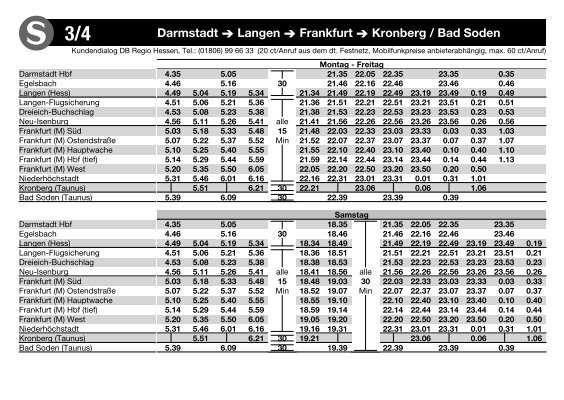
\includegraphics[width=.8\linewidth]{images/fahrplan-s3s4.jpg}
	\end{center}
\end{frame}

\begin{frame}{Fahrplanauskunftssysteme}
	\vspace{4em}
	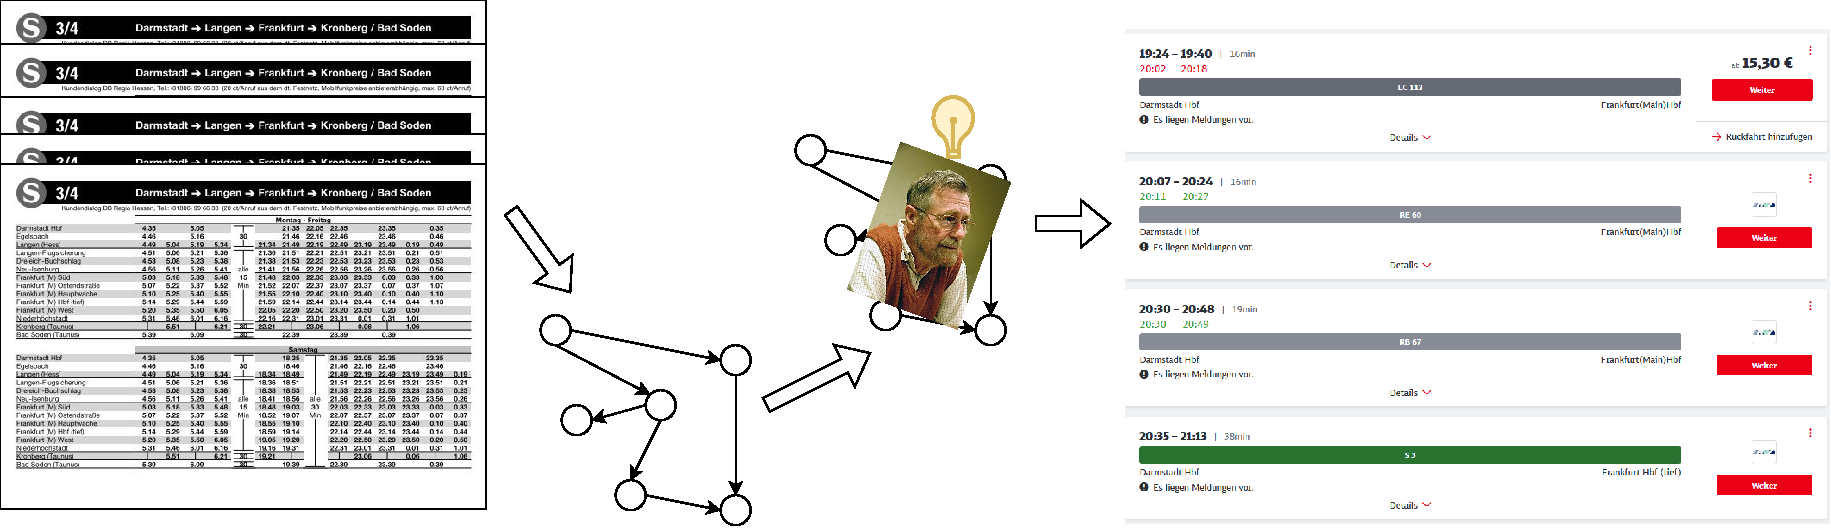
\includegraphics[width=\linewidth]{images/fahrplan-zu-auskunftssystem.pdf}
\end{frame}

\begin{frame}{Fahrplanauskunftssysteme}
	\vspace{3em}
	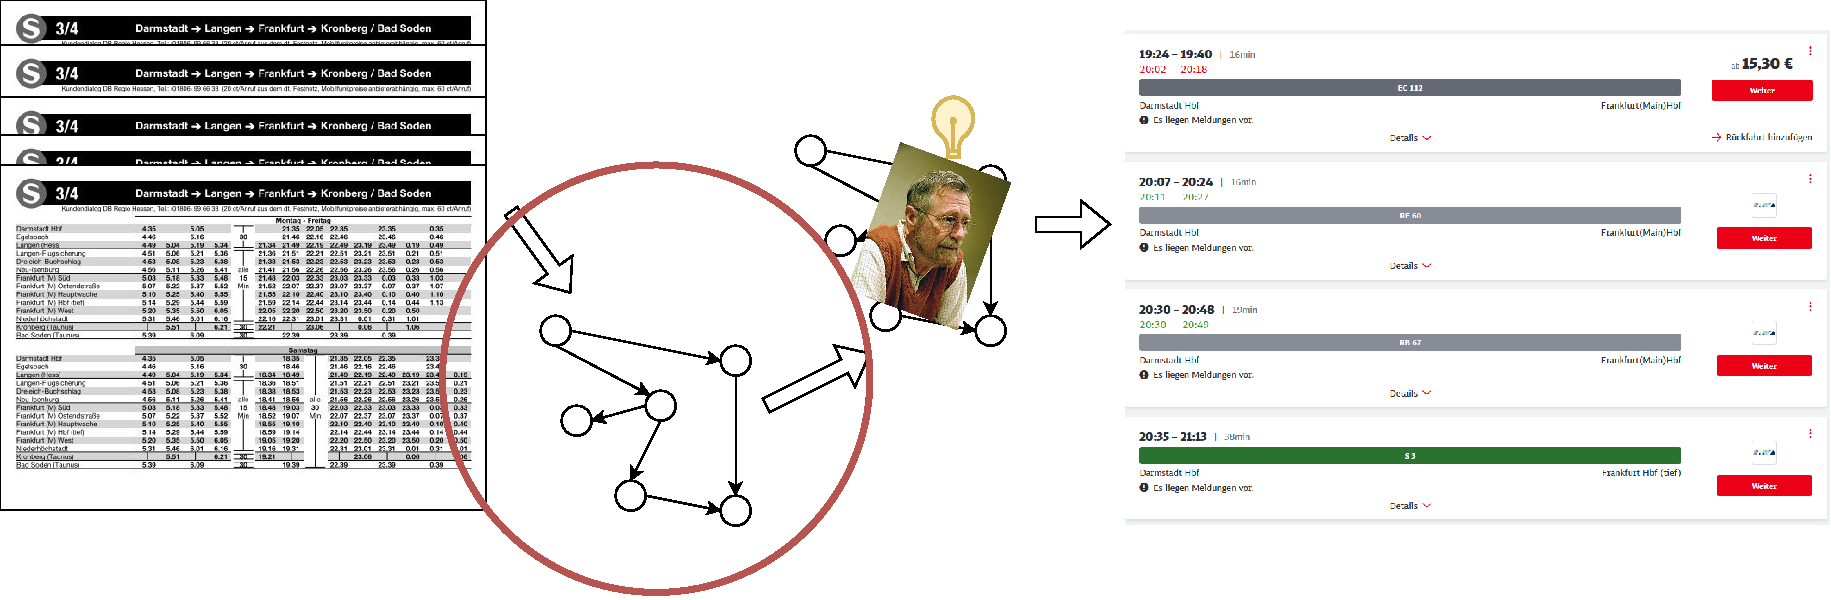
\includegraphics[width=\linewidth]{images/fahrplan-zu-auskunftssystem-2.pdf}
\end{frame}


\begin{frame}{Frage 1}
	\vspace{7em}
	\begin{center}
		\begin{Large}
			Wie wandle ich Fahrpläne zu Graphen um?
		\end{Large}
	\end{center}
\end{frame}

\begin{frame}{Frage 2}
	\vspace{6em}
	\begin{center}
		\begin{Large}
			Wie modelliere ich meinen Graphen, um das Earliest-Arrival Problem zu lösen?
		\end{Large}
	\end{center}
\end{frame}


\begin{frame}{Überblick}
	\begin{itemize}
		\item Grundlagen
	\end{itemize}
	\vspace{1em}
	\begin{itemize}
		\item Das 1. Graphenmodell
		\begin{itemize}
			\item Verfeinerungen
		\end{itemize}
	\end{itemize}
	\vspace{1em}
	\begin{itemize}
		\item Das 2. Graphenmodell
		\begin{itemize}
			\item Verfeinerungen
		\end{itemize}
	\end{itemize}
	\vspace{1em}
	\begin{itemize}
		\item Vergleiche
	\end{itemize}
	\vspace{1em}
	\begin{itemize}
		\item Zusammenfassung
	\end{itemize}
\end{frame}


\section{Terminologie}
\begin{frame}{1. Griff in die Terminologie-Kiste}
	\framesubtitle{Züge und Stationen}

	\begin{block}{}
		Was ist ein Zug?
	\end{block}
	
	\begin{center}
		\begin{tikzpicture}
			\node (img1) {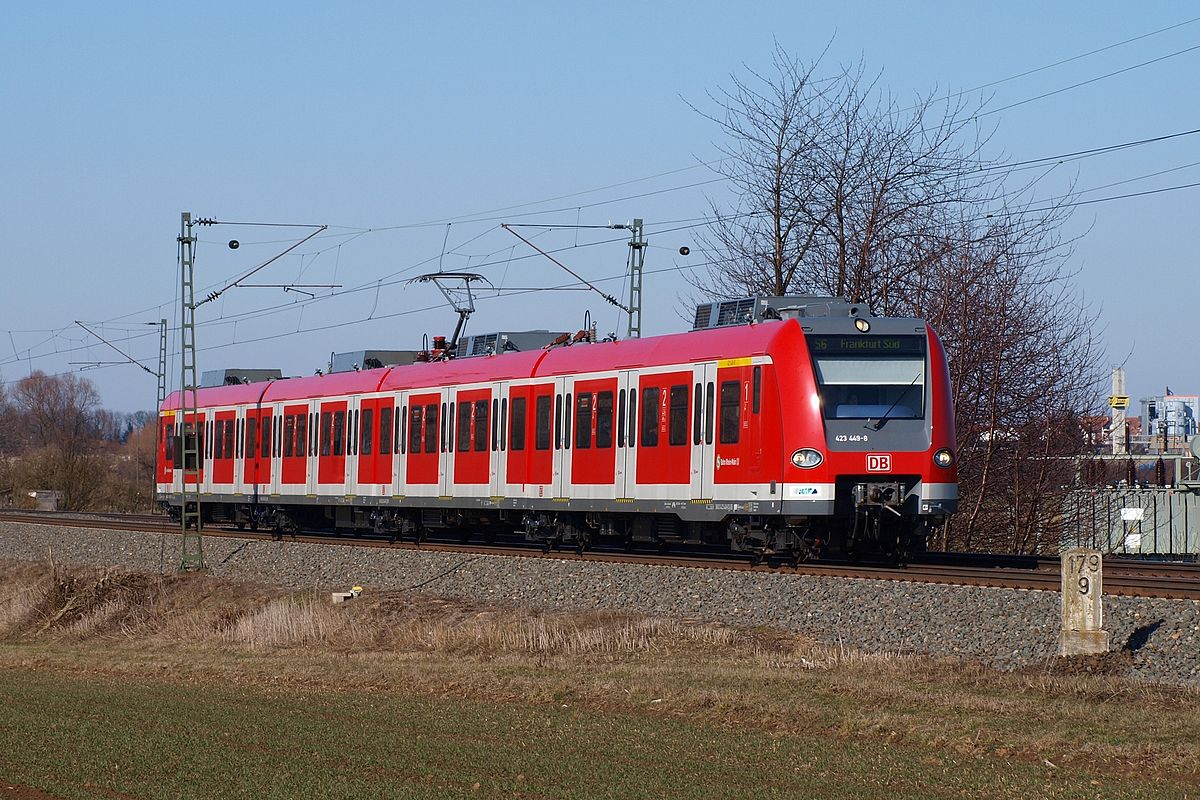
\includegraphics[height=4.5cm]{images/sbahn.jpg}};
			\pause
			\node (img2) at (img1.center) {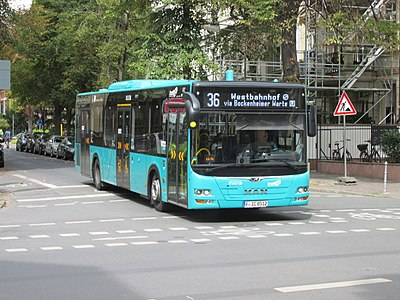
\includegraphics[height=4.5cm]{images/bus.jpg}};
			\pause
			\node (img3) at (img2.center) {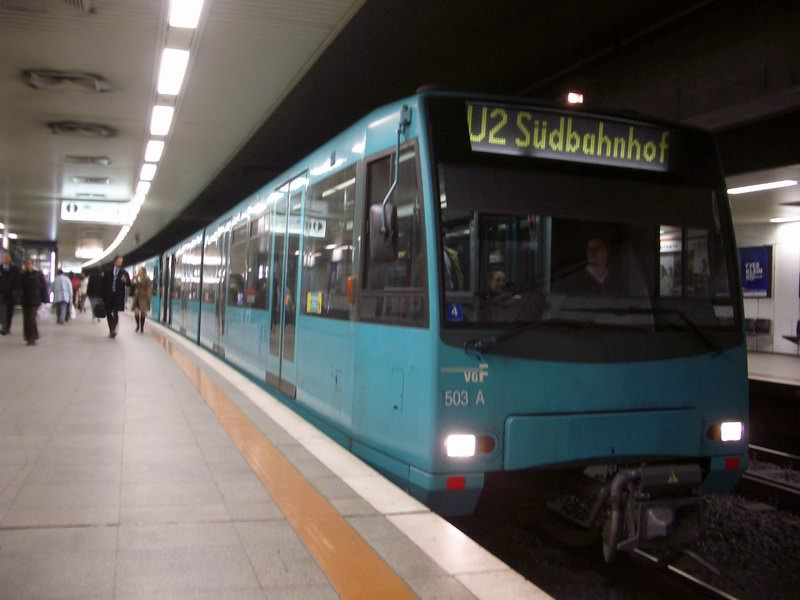
\includegraphics[height=4.5cm]{images/ubahn.jpg}};
			\pause
			\node (img4) at (img3.center) {\includegraphics[height=4.5cm]{images/fähre.jpg}};
		\end{tikzpicture}
	\end{center}
\end{frame}

\begin{frame}{1. Griff in die Terminologie-Kiste}
	\framesubtitle{Züge und Stationen}

	\begin{block}{}
		Was ist eine Station?
	\end{block}
	
	\begin{center}
		\begin{tikzpicture}
			\node (img1) {\includegraphics[height=4.5cm]{images/köppern.jpg}};
			\pause
			\node (img2) at (img1.center) {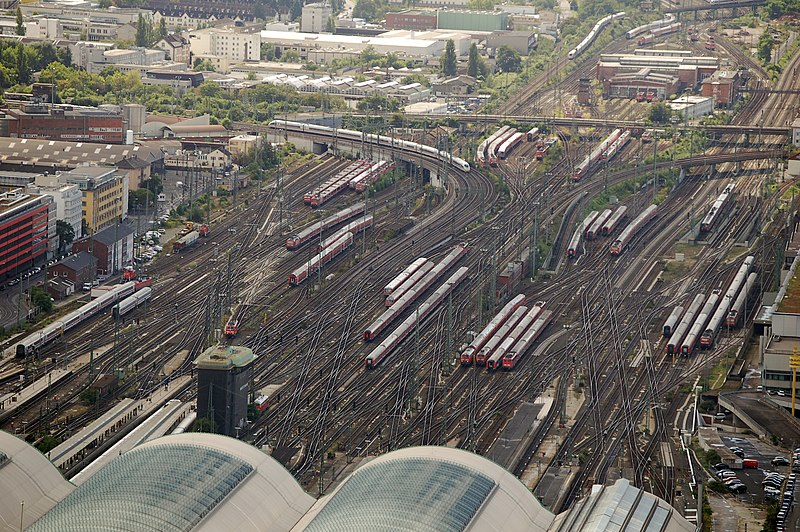
\includegraphics[height=4.5cm]{images/ffm.jpg}};
		\end{tikzpicture}
	\end{center}
\end{frame}


\begin{frame}{Größenordnungen}
	\begin{itemize}
		\item Ein paar Zahlen im Jahr 2008 (\textbf{nur} Züge):
	\end{itemize}

	\vspace{3em}
	\begin{center}
		\begin{tabular}{ c|c } 
			Anzahl & \\
 			\hline
 			Stationen & etwa\texttrademark{} 5000 \\
 			Züge & 68073 \\ 
 			Fußwege & 425 \\
		\end{tabular}
	\end{center}
\end{frame}


\subsection{Naive Ansätze}
\begin{frame}{Wie modelliere ich einen Fahrplan als Graphen?}
	\begin{itemize}
		\item Simple Idee: Knoten sind Stationen, Kanten sind Verbindungen 
	\end{itemize}
	
	\vspace{3em}
	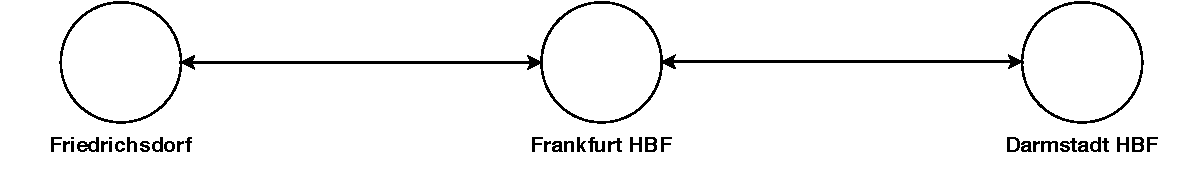
\includegraphics[width=\linewidth]{images/simple-approach.pdf}
	\vspace{3em}
	\begin{block}{}
		Was ist das Problem hier?
	\end{block}
\end{frame}

\begin{frame}{Wie modelliere ich einen Fahrplan als Graphen?}
	\begin{itemize}
		\item Wir müssen irgendwie Zeitverhältnisse innerhalb des Graphen darstellen!
	\end{itemize}
	
	\begin{center}
		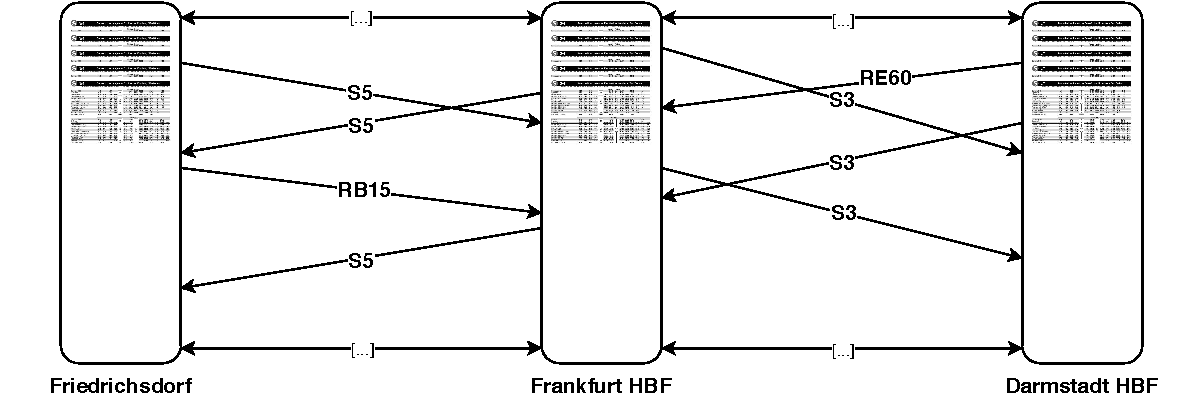
\includegraphics[width=\linewidth]{images/simple-approach-timed.pdf}
	\end{center}

	\begin{block}{}
		Was ist das Problem hier?
	\end{block}
\end{frame}

%\begin{frame}
%	\begin{itemize}
%		\item Wir müssen irgendwie Zeitverhältnisse innerhalb des Graphen darstellen!
%	\end{itemize}
%	
%	\begin{center}
%		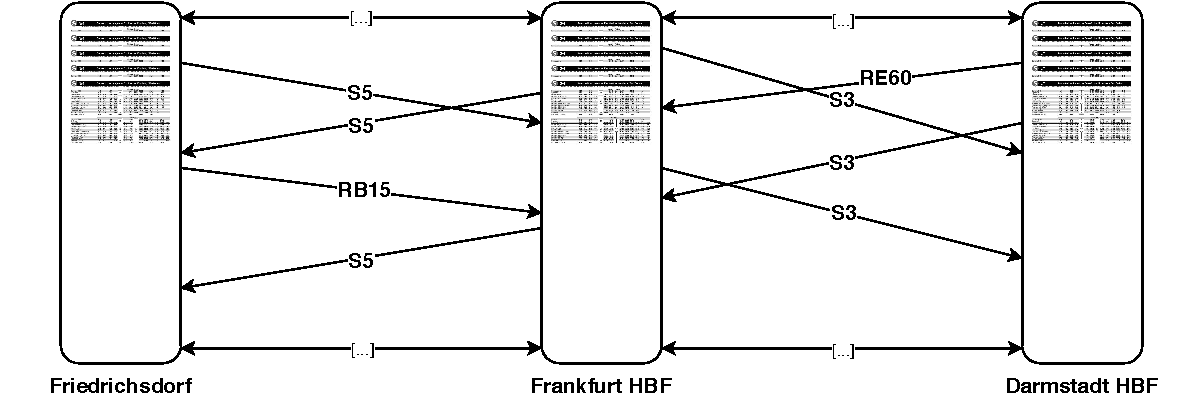
\includegraphics[width=\linewidth]{images/simple-approach-timed-2.pdf}
%	\end{center}
%
%	\begin{block}{}
%		Was ist das Problem hier?
%	\end{block}
%\end{frame}

\begin{frame}{Probleme}
	\framesubtitle{Die es zu lösen gilt...}
	\begin{itemize}
		\item Zeitverhältnisse im Graphen \pause
		\item \textbf{Takt}fahrpläne \pause
		\item Umstiege bzw. Umsteigezeiten \pause		
		\item Fußwege zwischen / innerhalb von Stationen \pause
		\item \sout{Intermodalität}
	\end{itemize}
	
	\vspace{6em}
	\begin{block}{Zwei gängige Modelle}
		Time-Expanded vs. Time-Dependent
	\end{block}
\end{frame}




















